\section{Implementation of relational operators}

\begin{figure}[h!]
		\centering
		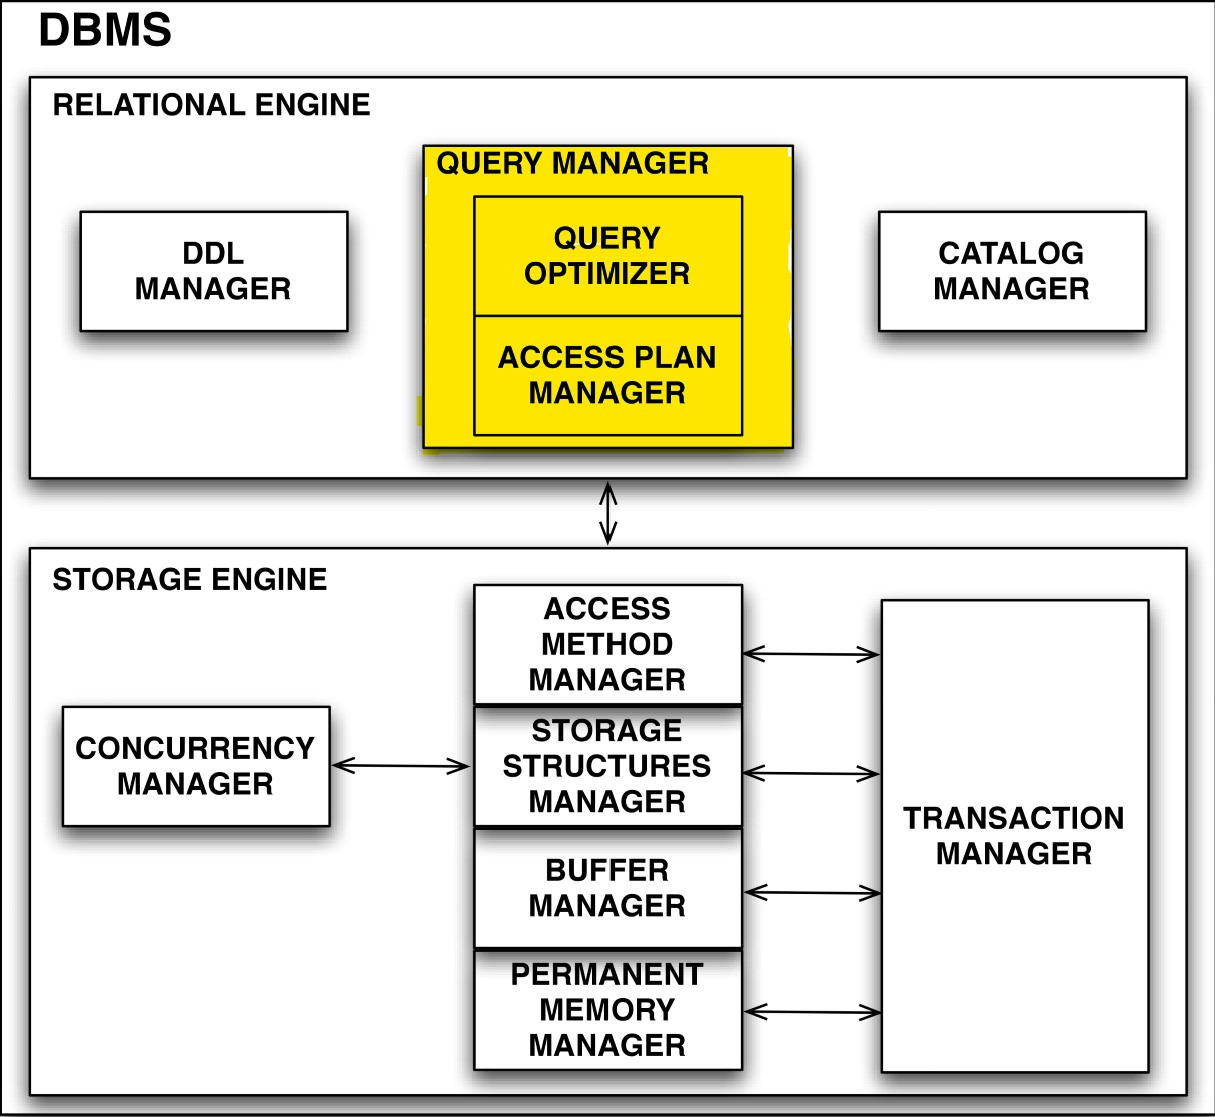
\includegraphics[scale = 0.7]{img/relop1.jpg}
		\label{part6}
\end{figure}

This chapter focuses on the Query Manager, one of the critical components of any DB system, and, in particular, on the algorithms for evaluating relational algebra operations, and how to estimate their cost and size.

\subsection{Assumptions and notation}

\subsubsection{Physical data organization}

\begin{itemize}
    \item each relation has attributes without null values, and it is stored in a heap file, or with the primary organization index sequential. 
    \item to make the operations on relations more efficient, \textbf{indexes} on one or more attributes are used. The indexes are organized as a B+–tree and those for non-key attributes are inverted indexes. We also distinguish two types of indexes:
    \begin{itemize}
        \item a \textbf{clustered index} is built on one or more attributes of a relation sorted on the index key. A relation can only  have one clustered index;
        \item an \textbf{unclustered index} is built on one or more attributes which are not used to sort a relation
    \end{itemize} 
\end{itemize}

\subsubsection{Physical query plan operators}

\begin{tcolorbox}
The \textbf{query optimizer} has the task of determining how to execute a query in an “optimal” way, by considering the physical parameters involved, such as the size of the relations, the data organization and the presence of indexes.
\end{tcolorbox}

 The problem is particularly difficult because, as we will see later, each relational algebra operator can be implemented in different ways and the query optimizer must use appropriate strategies to estimate the costs of the alternatives and choose the one with lowest cost. 
 
 The algorithm chosen by the optimizer to execute a query is represented as a tree, which is called \textbf{physical query plan}. The nodes of this tree are physical operators, each of which is a particular implementation of an operator of the \textbf{relational algebra extended on multisets}. This extension of relational algebra allows to manage multisets, which is what SQL table represent, and for this reason it supports the following operations:

 \begin{itemize}
     \item \textbf{projection with duplicates}: $\pi_X^b(O)$, with $X$ attributes of $O$;
     \item \textbf{duplicate elimination}: $\sigma(O)$;
     \item \textbf{sorting}, used by the SQL statement ORDER BY: $\tau_X(O)$;
     \item \textbf{multiset union, intersection and difference}.
 \end{itemize}

 An example of physical query plan:

 \begin{figure}[h!]
		\centering
		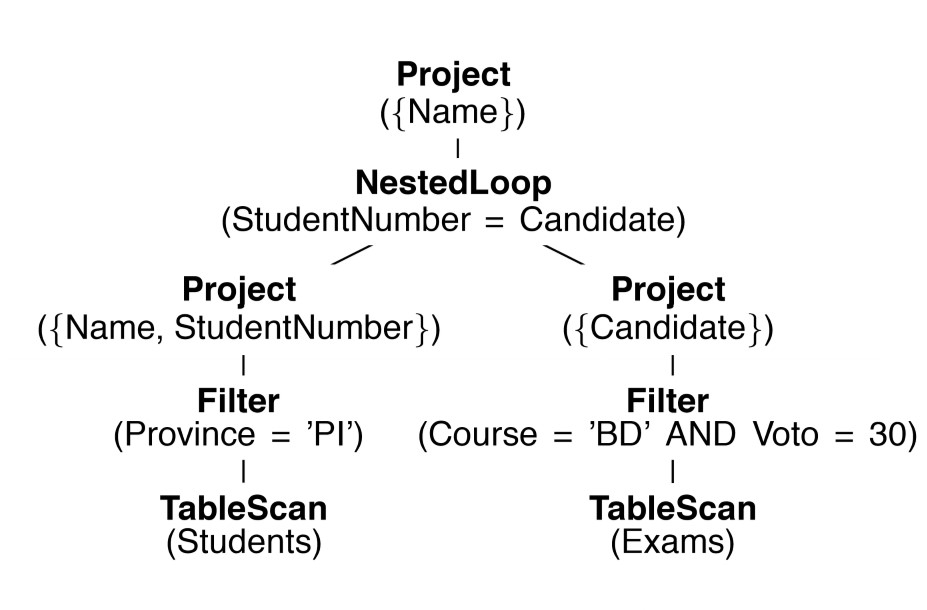
\includegraphics[scale = 0.9]{img/relop2.jpg}
		\label{part6}
\end{figure}

 
Each DBMS has its own \textbf{physical operators} and, for simplicity, we will consider
those of the JRS system. 

\textbf{NOTE}: 
\begin{itemize}
    \item for each physical operator we estimate the data access cost $C$ and the cardinality of its result $E_{rec}$;
    \item physical operators, like the operators of relational algebra, return collections of records with a type that depends on the operator.
\end{itemize} 

\subsubsection{Physical query plan execution}

Physical operators are implemented as \textbf{iterators} that produce the records of the result one at a time on request. An iterator behaves as an object with state, and methods \textit{open}, which initializes the process of getting records, \textit{isDone}, which tests if the iterator has more data to return, \textit{next}, \textit{reset} and \textit{close}.
For example, a physical query plan with root \textit{Plan} is executed as follows:

\begin{figure}[h!]
		\centering
		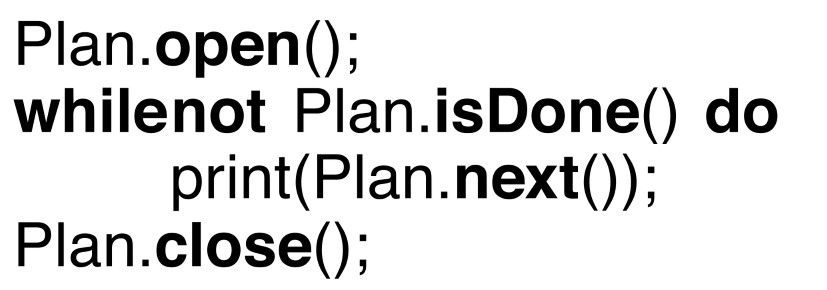
\includegraphics[scale = 0.7]{img/relop3.jpg}
		\label{part6}
\end{figure}

Physical operators are either \textbf{blocking} or \textbf{non-blocking}. A blocking operator, when is opened, must call next exhaustively on its operands before returning its first (or next) record (e.g. the sort operator)

\subsubsection{Cost model}
The \textbf{cost estimate} $C$ of executing a physical operator is given by the number of pages read from or written to the permanent memory to produce the result

\subsection{Physical operators for relation (\textit{R})}
The records of a relation can be retrieved with any of the following operators:

\begin{itemize}
    \item \textbf{TableScan(R)}: it returns the record of $R$ in the order they're stored. This operator belongs to all primary organizations. The cost is:

    $$
    C = N_{\text{pag}(R)}
    $$

    \item \textbf{SortScan(R,A\_i)}: it return the records of $R$ sorted in ascending order according to the attribute $A_i$.
    \begin{itemize}
        \item sorting is done with \textit{merge sort} algorithm
        \item in general, the operator's cost depends on $N_{\text{pag}(R)}$, the number of pages $B$ available in the buffer and the implementation of the \textit{merge sort} algorithm;
        \item this operator is available for all possible primary organizations.
    \end{itemize}
    We assume that the cost is:

    $$
    C = 3N_{\text{pag}(R)}
    $$
    , under the condition that $N_{\text{pag}(R)} < B^2$

    \item \textbf{IndexScan(R,I)}: it returns the records of $R$ sorted in ascending order according to the attribute $A_i$ values of the index $I$. The cost depends both on the type of index and on the type of attribute on which it is defined:

    $$
    C = \begin{cases}
        N_{\text{leaf}}(I) + N_{\text{pag}(R)} & \mbox{if} \text{ I is clustered} \\
        N_{\text{leaf}}(I) + N_{\text{rec}(R)} & \mbox{if} \text{ I is unclustered} \\
        N_{\text{leaf}}(I) + \ceil*{N_{\text{key}}(I) \times \phi (\ceil*{N_{\text{rec}}(R)/N_{\text{key}}(I)}, N_{\text{pag}(R))}} & \mbox{if} \text{ I is an inverted index}
        \end{cases}
    $$

    Note that $N_{\text{leaf}}(I)$ represents the cost of accessing the index, while the other addend represents the cost for accessing the data, and it depends on the nature of the index $I$.

    \item \textbf{IndexSequentialScan(R,I)}: it returns the records of $R$, stored with primary organization \textit{index sequential I}, sorted in ascending order on the primary key values. The cost is:

    $$
    C = N_{\text{leaf}}(I)
    $$
    
\end{itemize}

\textbf{NOTE}: in all the cases, the cardinality of the result is:

$$
E_{\text{rec}} = N_{\text{rec}(R)}
$$

\subsection{Physical operator for projection with duplicates ($\pi^b$)}

\begin{itemize}
    \item \textbf{Project(O,A\_i)}: it returns the records of the projections of the records of $O$ over the attributes ${A_i}$. The cost is:

    $$
    C = C(O)
    $$
    , if there are no subqueries.

    The cardinality of the result is:

    $$
    E_{\text{rec}} = E_{\text{rec}(O)}
    $$

    This operator is always available.

    \item \textbf{IndexOnlyScan(R,I,A\_i)}: it returns the sorted records of $\pi_{A_i}^b(R)$ by using the index $I$ on the attributes $A_i$. The cost is:

    $$
    C = N_{\text{leaf}}(I)
    $$

    , while the cardinality of the result is:

    $$
    E_{\text{rec}} = N_{\text{rec}(R)}
    $$
    
\end{itemize}

\subsection{Physical operators for duplicate elimination ($\delta$)}

\begin{itemize}
    \item \textbf{Distinct(O)}: returns the record of $O$ sorted and without duplicates, i.e. it converts $O$ from a multiset to a set. The crucial precondition is that the records of $O$ are sorted. The cost is:

    $$
    C = C(O)
    $$

    \item \textbf{HashDistinct(O)}: it eliminates the duplicates of $O$ using an hash technique. Suppose that we have $B + 1$ pages in the buffer to perform duplicate elimination, then this technique is composed of two phases that use two different hash functions:
    
    \begin{itemize}
        \item the \textit{partitioning phase}, in which the first hash function $h_i$ is applied to each record of $O$ to distribute the records uniformly in the $B$ pages: the result are $B$ files, each containing a collection of records with the same hash value;
        \item the \textit{duplicate elimination phase}, in which the second hash function $h_2$ is applied to all record attributes of each page of each partition in order to eliminate the duplicates.
    \end{itemize}

    The cost is:

    $$
    C = C(O) + 2 \times N_{\text{pag}(O)}
    $$
    
\end{itemize}

We notice that the \textit{HashDistinct} technique has the same cost of the \textit{Distinct} tecnhique with the sorting of the operand records, but it does not procude a sorted result.

\subsection{Physical operators for selection ($\sigma$)}

\begin{itemize}
    \item \textbf{Filter(O, $\psi$)}: it returns the records of $O$ satisfying the condition $\psi$. The cost is:

    $$
    C = C(O)
    $$

    This operator is always available.

    \item \textbf{IndexFilter(R,I,$\psi$)}: it returns the records of $R$ satisfying the condition $\psi$ with the use of the index $I$, defined on attributes $\psi$ ; more specifically:
    \begin{itemize}
        \item it uses the index to find the sorted set of RIDs satisfying the condition, using \textbf{RIDIndexFilter(I, $\psi$)};
        \item retrieves the records of $R$ using \textbf{TableAccess(O,R)}.
    \end{itemize}

    The cost is given by:

    $$
    C = C_I + C_D
    $$
    , where $C_I$ and $C_D$ depend on the type of index and the type of attributes on which it is defined.

    \item \textbf{IndexSequentialFilter(R,I,$\psi$)}: it returns the sorted records of $R$, stored with the primary organization \textit{index sequential I}, satisfying the condition $\psi$. The cost is:

    $$
    C = \ceil*{s_f(\psi) \times N_{\text{leaf}()I}}
    $$

    \item \textbf{IndexOnlyFilte(R,I,$A_i$,$\psi$)r}: it returns the sorted records of $\pi_{A_i}^b(\sigma_{\psi}(R))$, using only the index I. The cost is:

    $$
    C = \ceil*{s_f(\psi) \times N_{\text{leaf}()I}}
    $$

    \item \textbf{OrIndexFilter(R,{$I_i$,$\psi_i$ })}: it returns the records of $R$ satisfying the disjunctive condition $\psi = \psi_1 \lor \psi_2 \lor ... \lor \psi_n$ using the index $I_i$ for each $\psi_i$. More specifically:
    \begin{itemize}
        \item it uses the index to find a sorted union of the RID lists of records matching each terms $\psi_i$;
        \item retrieves the records of $R$.
    \end{itemize}
    The cost is:

    $$
    C = C_I + C_D
    $$
    , where 

    $$
    C_I = \ceil*{\sum\limits_{k = 1}^n C_I^k }
    $$

    and 

    $$
    C_D = \ceil*{\Phi (E_{\text{rec}} , N_{\text{pag}}(R))}
    $$

    \item \textbf{AndIndexFilter(R,{ $I_i$, $\psi_i$ })}: it returns the records of $R$ satisfying the conjunctive condition $\psi = \psi_1 \land \psi_2 \land ... \land \psi_n$ using the index $I_i$ for each $\psi_i$. More specifically:
    \begin{itemize}
        \item it uses the index to find a sorted intersection of the RID lists of records matching each terms $\psi_i$;
        \item retrieves the records of $R$.
    \end{itemize}
    The cost is:

    $$
    C = C_I + C_D
    $$
    , where 

    $$
    C_I = \ceil*{\sum\limits_{k = 1}^n C_I^k }
    $$

    and 

    $$
    C_D = \ceil*{\Phi (E_{\text{rec}} , N_{\text{pag}}(R))}
    $$
    
\end{itemize}

Picture \ref{relop4} and \ref{relop5} show two examples of access plans that are constructed from two simple queries: note that in the second query we can use IndexFilter because there's an index on the attribute $A$ and , but we cannot use IndexOnlyFilter because we have "SELECT *".

\begin{figure}[h!]
		\centering
		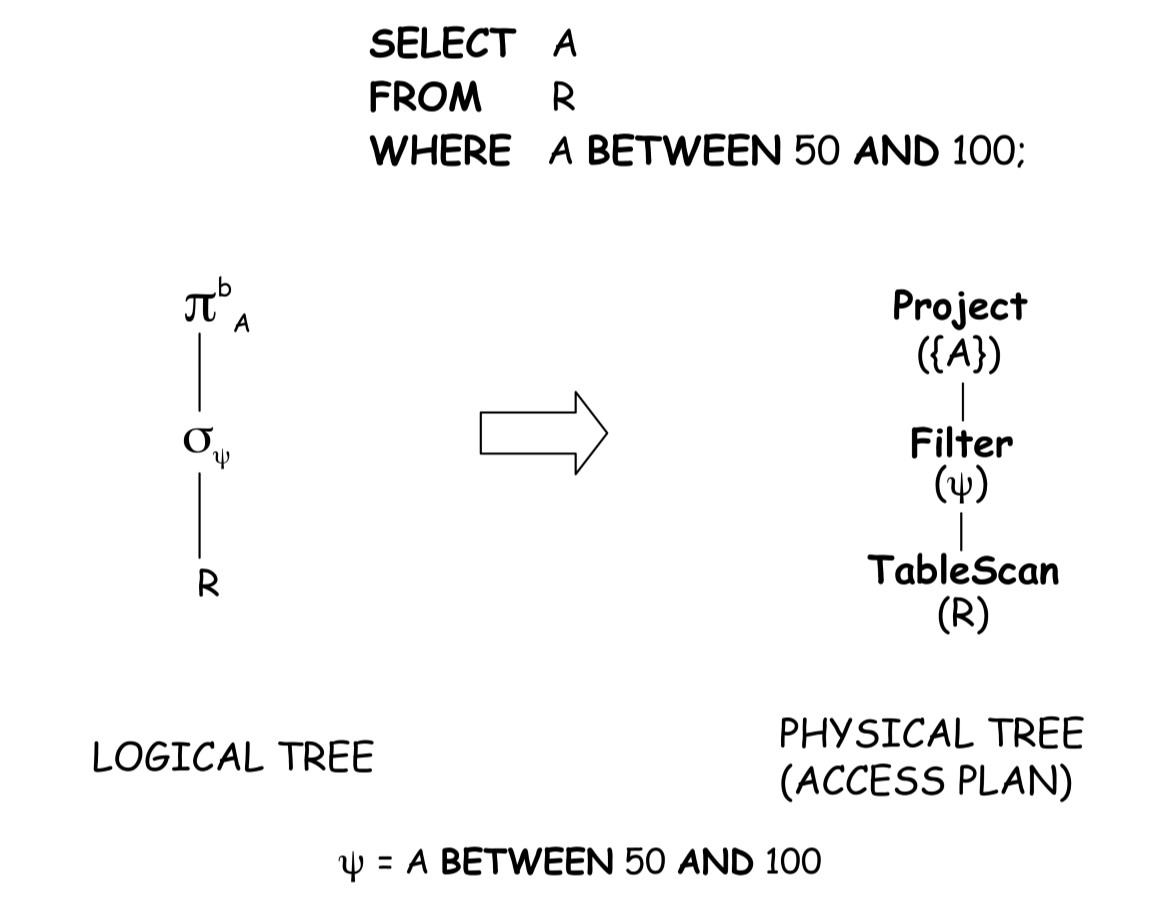
\includegraphics[scale = 0.7]{img/relop4.jpg}
		\label{relop4}
\end{figure}

\begin{figure}[h!]
		\centering
		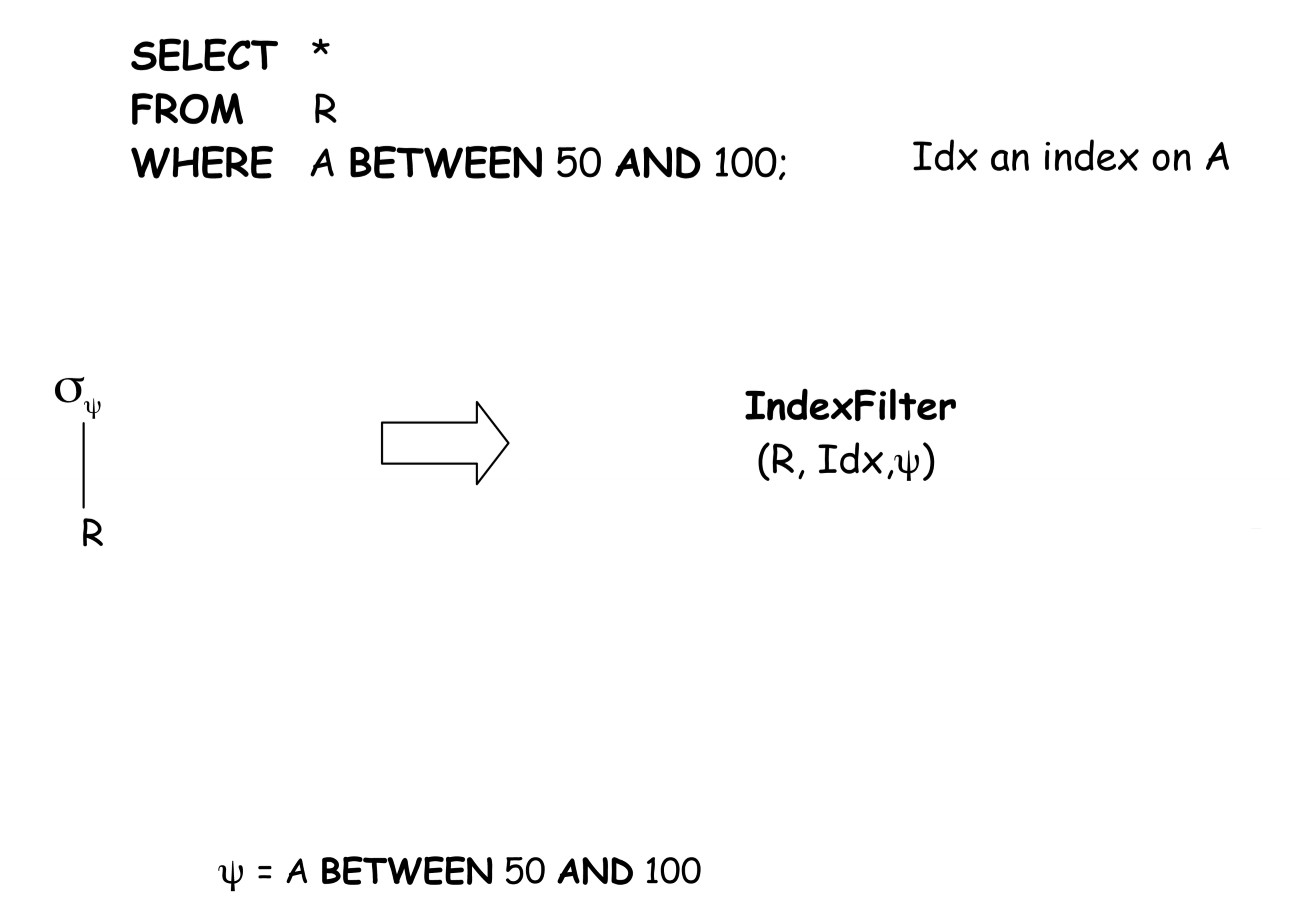
\includegraphics[scale = 0.7]{img/relop5.jpg}
		\label{relop5}
\end{figure}


\subsection{Physical operators for grouping ($\gamma$)}
The records of $R$ are partitioned according to their values in one set of attributes $A_i$, called the \textit{grouping attributes}. Then, for each group, the values in certain other attributes are aggregated with the functions $f_i$. The result of this operation is one record for each group. 
To execute the grouping of the operand $O$ result, the following physical operators are used, which differ in the way the records of $O$ are partitioned:

\begin{itemize}
    \item \textbf{GroupBy(O,$A_i$,${f_i}$)}: the records of $O$ are sorted on the grouping attributes $A\_i$, so that the records of each group are next to each other. Note that in the set ${f_i}$ there are the aggregation functions present in the SELECT and HAVING clauses. The cost is:

    $$
    C = C(O)
    $$

    \item \textbf{HashGroupBy(O,${A_i}$,${f_i}$)}: the records of $O$ are partitioned using an hash function on the attributes ${A_i}$:
    
    \begin{itemize}
        \item \textit{partitioning phase}: using the hash function $h_1$, a partition is created;
        \item \textit{grouping phase}: using the hash function $h_2$ to all grouping attributes, the records of each partition are grouped.
    \end{itemize}
    
    The cost is:

    $$
    C = C(O) + 2 \times N_{\text{pag}(O)}
    $$
    
\end{itemize}

Picture \ref{relop6} shows an example of GROUP BY query that is transformed into an access plan.


\begin{figure}[h!]
		\centering
		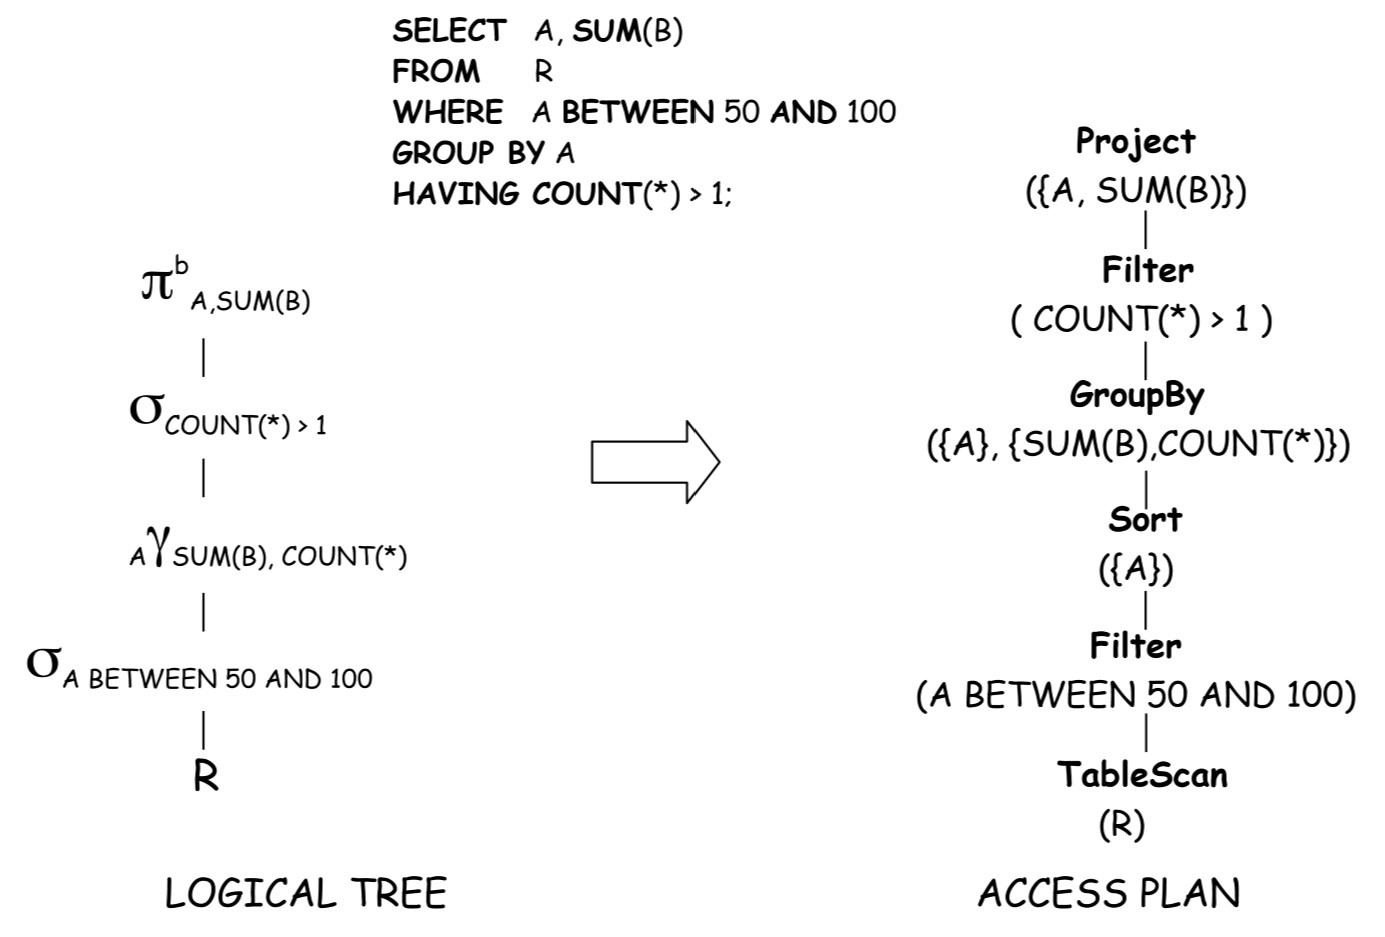
\includegraphics[scale = 0.8]{img/relop6.jpg}
		\label{relop6}
\end{figure}

\subsection{Physical operators for join ($\bowtie$)}
The JOIN operation can be considered as cartesian product + filter operation: the cartesian product crates all the possible pairs, while the filter operation removes the pairs in which the primary key does not match. However, if we have two sets $A$ and $B$, then the number of pairs is  $|A \times B|$, and most of them are discarded, so it is an inefficient operation. For this reason, the two possible options to optimize the JOIN operation is:

\begin{itemize}
    \item reduce the number of candidates using an index;
    \item reduce the cost of access, using the same number of candidates.
\end{itemize}

We only consider $O_E \bowtie_{\psi_J} O_I$, where:
\begin{itemize}
    \item $O_E$ is the external operand;
    \item $O_I$ is the internal operand;
    \item $\psi_J$ is the join condition.
\end{itemize}

\begin{itemize}
    \item \textbf{NestedLoop($O_E$, $O_I$ $\psi_J$)}:

    \begin{figure}[h!]
		\centering
		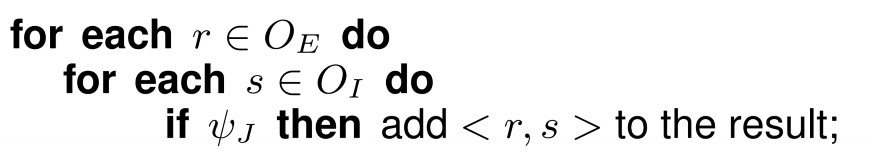
\includegraphics[scale = 0.8]{img/relop7.jpg}
		\label{relop6}
    \end{figure}

    The cost is:

    $$
    C = C(O_E) + E_{\text{rec}(O_E)} \times C(O_I)
    $$
    , but the order of the loops matter! From the cost function we can see that all the pages of the internal operand are accessed for each page of the external operand, so it is more convenient to have as external operand the relation with more tuples.

    \item \textbf{PageNestedLoop($O_E$, $O_I$, $\psi_J$)}: this operator exploit the buffer in order to reduce the number of disk accesses: in particular, the result of $O_I$ is scanned once per page of $O_E$, instead of per each record of $O_E$. For this reason, the larger the page size, the better in terms of computational complexity.

    \begin{figure}[h!]
		\centering
		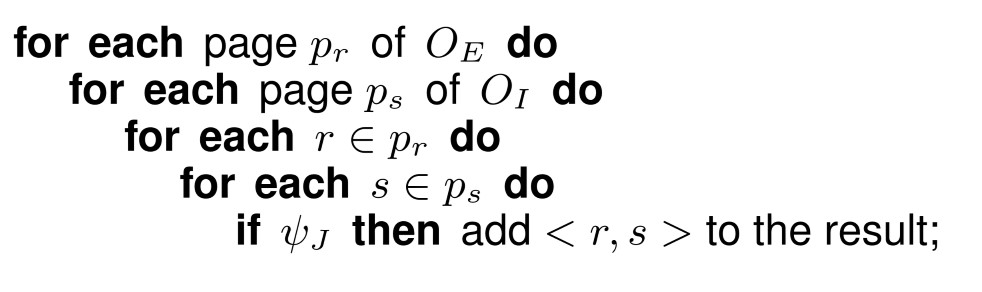
\includegraphics[scale = 0.8]{img/relop8.jpg}
		\label{relop6}
    \end{figure}

    The cost is:

    $$
    C = C(O_E) + N_{\text{pag}(O_E)} \times C(O_I)
    $$

    In this case, the algorithm cost is lower when the external relation is the one with fewest pages.
    
\end{itemize}

\textbf{NOTE}:
\begin{itemize}
    \item both NestedLoop and PageNestedLoop do not have any knowledge about the predicates, so no index is used;
    \item PageNestedLoop is better than NestedLoop, being $N_{\text{pag}(O_E)} < N_{\text{rec}(R)}$, but it does not produce a sorted result.
\end{itemize}

\begin{itemize}
    \item \textbf{IndexNestedLoop($O_E$, $O_I$, $\psi_J$)}: in this case we have some knowledge about the predicates, in particular we can use an index in order to filter the records and reduce the number of candidates. However, the preconditions are:
    \begin{itemize}
        \item the join is an \textit{equi-join}. It can be used not only for equi-join, provided that it has an access method for the predicate;
        \item there is an IndexFilter on the internal operand.
    \end{itemize}

    \begin{figure}[h!]
		\centering
		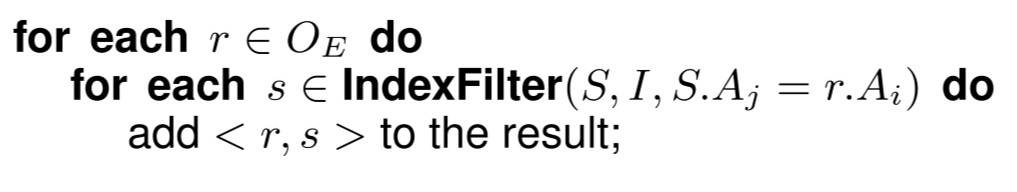
\includegraphics[scale = 0.8]{img/relop9.jpg}
		\label{relop6}
    \end{figure}

    The cost is:

    $$
    C = C(O_E) + E_{\text{rec}(O_E)} \times (C_I + C_D)
    $$
    , where $(C_I +C_D)$ is the cost to retrieve the matching records of $S$ with a record of $O_E$ that depends on the index type.

    \item \textbf{MergeJoin($O_E$, $O_I$, $\psi_J$)}: in this case the precondition are:

    \begin{itemize}
        \item the join is an \textit{equi-join};
        \item $O_E$ and $O_I$ are sorted on the join attributes $O_E.A_i$ and $O_I.A_i$;
        \item the join attribute $O_E.A_i$ is a key.
    \end{itemize}

    The cost is:

    $$
    C = C(O_E) + C(O_I)
    $$

    This operator is efficient provided that $O_E$ and $O_I$ are sorted, otherwise we have to consider some additional costs.

    \item \textbf{HashJoin($O_E$, $O_I$, $\psi_J$)}: similarly to HashDisinct and HashGroupBy, this operator computes the join in two phases:
    \begin{itemize}
        \item in the \textit{partitioning phase}, the records of $O_E$ and $O_I$ are partitioned using the first hash function $h_1$ applied to the join attributes. If two tuples are joined, they belong to the same partition but in different pages.

        \begin{figure}[H]
		\centering
		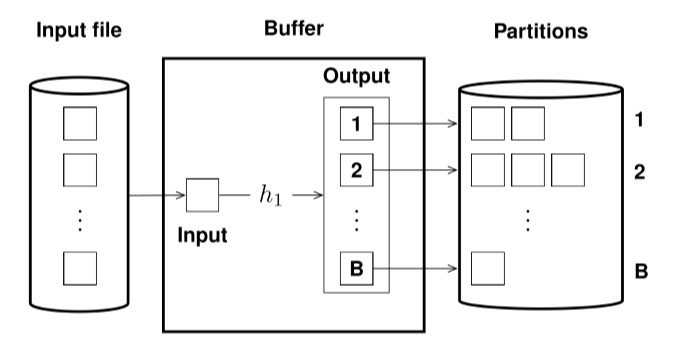
\includegraphics[scale = 0.8]{img/relop10.jpg}
		\label{relop6}
        \end{figure}

        
        \item in the \textit{probing phase}, for each partition $B_i$ 
        \begin{itemize}
            \item the records of $O_E$ are read and inserted into buffer hash table with $B$ pages using the function $h_2$ applied to the join attribute values;
            \item the records of $O_I$ are read one page at a time, and which of them join with those of $O_E$ is checked with $h_2$, and they're added to the result;
        \end{itemize}

        \begin{figure}[H]
		\centering
		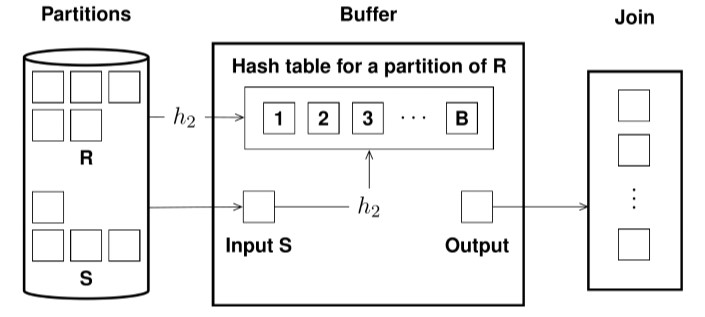
\includegraphics[scale = 0.9]{img/relop11.jpg}
		\label{relop6}
        \end{figure}

    \end{itemize}

    The costs are:

    $$
    C_{\text{partitioning}} = C(O_E) + C(O_I) + N_{\text{pag}(O_E)} + N_{\text{pag}(O_I)}
    $$

    $$
    C_{\text{probing}} = N_{\text{pag}(O_E)} + N_{\text{pag}(O_I)}
    $$

    , so the total cost is:

    $$
    C = C(O_E) + C(O_I) + 2 \times (N_{\text{pag}(O_E)} + N_{\text{pag}(O_I))}
    $$
    
\end{itemize}

In general, since $O_E \bowtie_{\psi_J} O_I = \sigma_{\psi_J}(R \times S)$, the \textbf{cardinality of the result} is :

$$
E_{\text{rec}} = \ceil*{s_f(\psi_J) \times E_{\text{rec}(O_E)} \times E_{\text{rec} (O_I) }  }
$$

Pictures \ref{relop12} and \ref{relop13} show two examples of join queries that are trasformed into access plans.

\begin{figure}[h!]
		\centering
		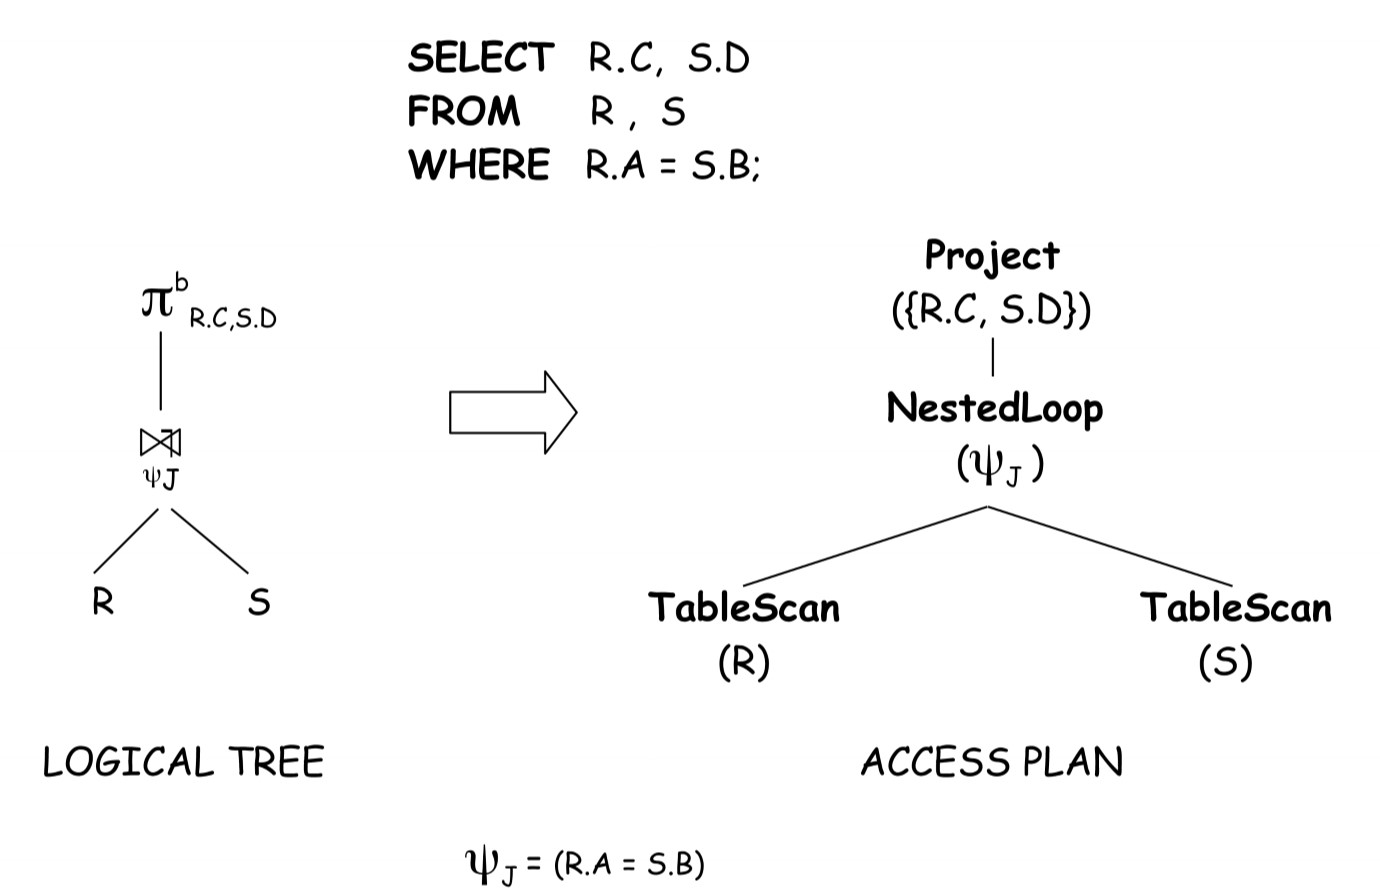
\includegraphics[scale = 0.7]{img/relop12.jpg}
		\label{relop12}
\end{figure}


\begin{figure}[h!]
		\centering
		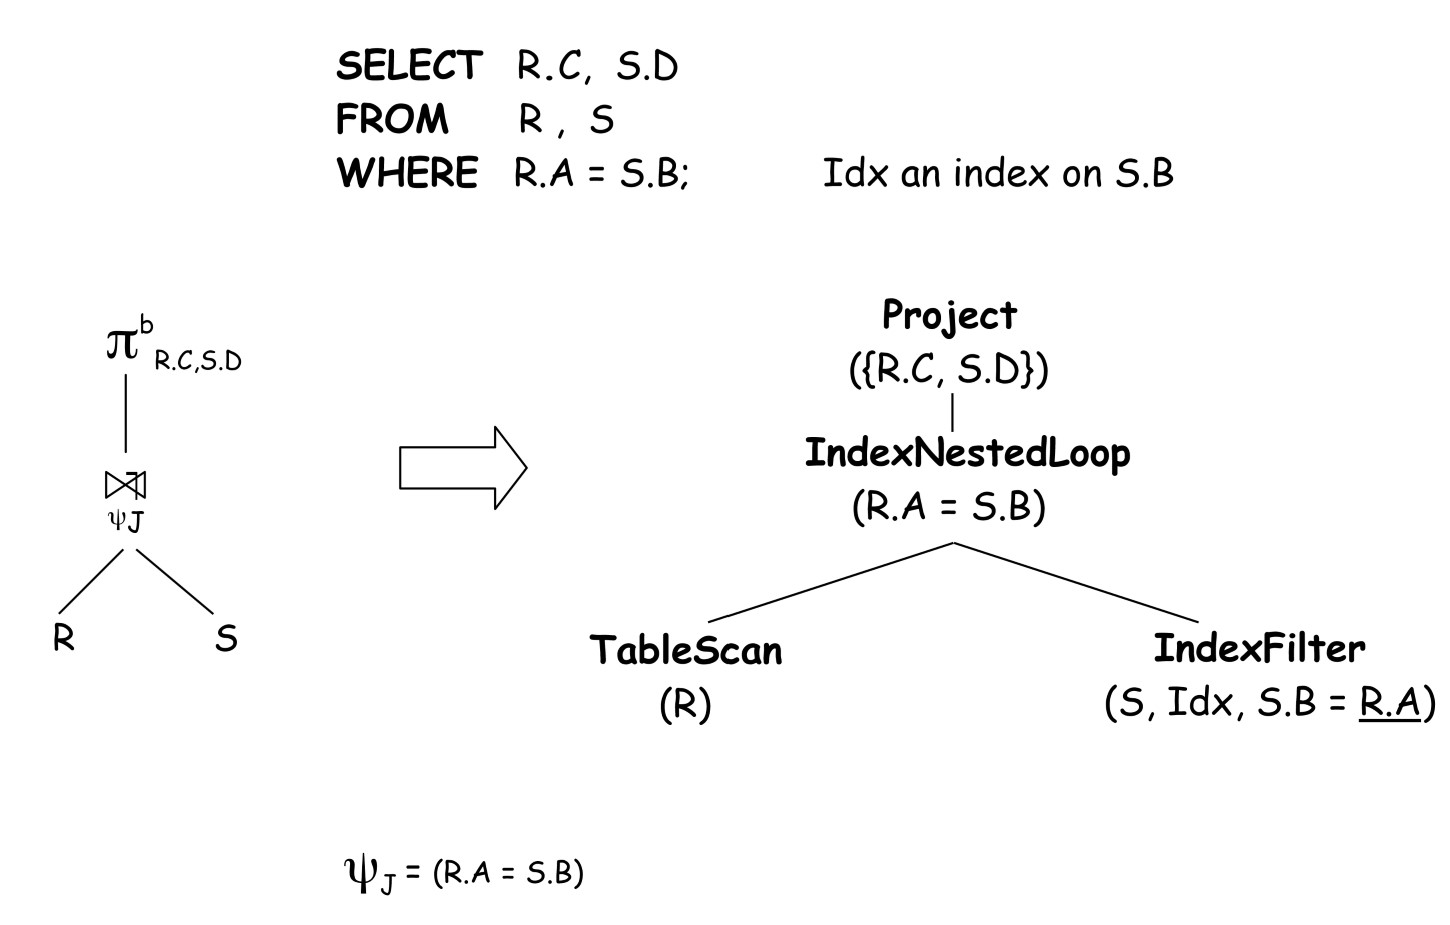
\includegraphics[scale = 0.7]{img/relop13.jpg}
		\label{relop13}
\end{figure}

\subsection{Physical operators for set and multiset operations}

\begin{itemize}
    \item \textbf{Union($O_E$,$O_I$)}, \textbf{Except($O_E$,$O_I$)} and \textbf{Intersect($O_E$,$O_I$)} require that the operand are sorted and do not have any duplicate element. In this case the cost is:

    $$
    C = C(O_E) + C(O_I)
    $$

    \item \textbf{UnionAll($O_E$,$O_I$)}, \textbf{ExceptAll($O_E$,$O_I$)} and \textbf{IntersectAll($O_E$,$O_I$)} do not eliminate duplicates, so they implement the multiset operations. The cost is:

    $$
    C = C(O_E) + C(O_I)
    $$
    
\end{itemize}